%!TEX root = 497Notes-Temple.tex

\section{MgNet, pre-act ResNet, variants and generalizations}\label{sec:relation}
%\subsection{Some properties of MgNet}
%So, this MgNet is corresponded to the multigrid methods 
%with iteration in function space. A natural idea is that there is also a dual version of 
%MgNet similar with the multigrid methods with iteration in dual space.
The MgNet model algorithm is one very basic and it can be generalized
in many different ways. It can also be used as a guidance to modify and 
extend many existing CNN models. 

The following result show how MgNet is related to the pre-act ResNet \cite{he2016identity}. 
\begin{theorem}\label{thm:mgnet1}
The MgNet model Algorithm \ref{alg:mgnet}, 
admits the following identities
\begin{equation}\label{dualmgnet}
r^{\ell, i} = r^{\ell, i-1} -  A^{\ell} \circ \sigma \circ B^{\ell,i}\circ \sigma (r^{\ell,i-1}), \quad i = 1:\nu_\ell, \\
\end{equation}
where
\begin{equation}
  \label{eq:5}
	r^{\ell,i} = f^{\ell} - A^{\ell} \ast u^{\ell,i}.   
\end{equation}
Furthermore, \eqref{dualmgnet} represents pre-act ResNet~\cite{he2016identity} 
as shown before.
\end{theorem}

\begin{proof}
	Because of the linearity of $A^\ell$ and invariant within the same grid $\ell$, 
	we can apply $A^\ell$ on both sides of \eqref{mgnet} and minus with
	$f^\ell$, thus we have
	$$
	f^{\ell} - A^{\ell} \ast u^{\ell,i} = f^{\ell} - A^\ell \ast u^{\ell,i-1} -
	A^{\ell} \ast \sigma \circ B^{\ell,i}\circ \sigma (f^\ell - A^\ell \ast u^{\ell,i-1}).
	$$
This finish the proof with definition in \eqref{eq:5}.
\end{proof}

The above result is very simple but critically important.
In view of Theorem \ref{thm:mgnet1}, it shows how multigrid and 
CNN are intimately related. Furthermore, it provides a different version
of iResNet, which can be viewed as the dual version of the original pre-act ResNet.
This relation is quit similar with the dual relation of $u$ and $f$
in multigrid method \cite{xu2017algebraic}.
\begin{lemma}\label{thm:mgnet2} 
	The ResNet~\cite{he2016deep} step
 	 as in \eqref{eq:ResNet} 
%	\begin{equation}\label{resnet}
%	f^{\ell,i} = \sigma( f^{\ell, i-1} - \xi^{\ell,i} \circ \sigma \circ \eta^{\ell,i} (f^{\ell,i-1}) ).
%	\end{equation}
admits the following relation:
%(which resembles closely with \eqref{dualmgnet}) 
\begin{equation}\label{tilde-resnet}
\tilde r^{\ell,i+1} =\sigma(\tilde r^{\ell,i}) -
A^{\ell,i} \ast \sigma \circ B^{\ell,i}\ast \sigma( \tilde r^{\ell,i}),
\end{equation}
where
\begin{equation}\label{tilde-f}
\tilde r^{\ell,i} = r^{\ell, i-1} -A^{\ell,i} \ast \sigma \circ B^{\ell,i} \ast r^{\ell,i-1}.
\end{equation}
\end{lemma}
\begin{proof}
%	Now, we will establish the connection between classical ResNet and MgNet. 
	First, we apply $ A^{\ell,i+1} \circ \sigma \circ B^{\ell,i+1}$ 
	on the both sides of \eqref{eq:ResNet} and get
	\begin{equation}\label{resnet1}
	A^{\ell,i+1} \ast \sigma \circ B^{\ell,i+1} \ast r^{\ell,i} = 
	A^{\ell,i+1} \ast \sigma \circ B^{\ell,i+1}\ast \sigma( \tilde r^{\ell,i} ).
	\end{equation}
	Minus by $r^{\ell,i}$ on the both sides and recall the definition in \eqref{tilde-f}, we have
	\begin{equation*}
	\tilde r^{\ell,i+1} = r^{\ell,i} - A^{\ell,i+1} \ast \sigma \circ B^{\ell,i+1}\ast \sigma( \tilde r^{\ell,i}).
	\end{equation*}
	By the definition of $r^{\ell,i} = \sigma(\tilde r^{\ell,i})$, we finish this proof.
\end{proof}

We call the above form \eqref{tilde-resnet} as
$\sigma$-ResNet, similar to the MgNet we replace $A^{\ell,i}$ by $A^{\ell}$  and get 
the next Mg-ResNet form as:
\begin{equation}\label{mg-resnet}
r^{\ell,i} =\sigma(r^{\ell,i-1}) -
A^{\ell} \ast \sigma \circ B^{\ell,i}\ast \sigma(r^{\ell,i-1}).
\end{equation}

If we take these pooling and prolongation operators
as discussed in the previous sections and focus on 
the iterative forms on a certain grid $\ell$, we may
compare them all as:
\begin{table}[!htbp]
	\caption{Comparison for all iterative forms }
	\label{comparison-ALL}
	\begin{center}%\scriptsize
		\resizebox{1.0\textwidth}{!}{
			\begin{tabular}{|c|c|c|}
				\hline
				Primal-Dual & Model & Iterative form \\
				\hline
				\multirow{3}{*}{Feature space} & Abstract-MgNet & Solving $A^\ell(u^\ell) = f^\ell$ \\
				\cline{2-3}
				& General-MgNet & $u^{\ell,i} = u^{\ell, i-1} + B^{\ell,i} (f^\ell - A^{\ell}(u^{\ell,i-1}))$ \\
				\cline{2-3}
				& {MgNet} & $u^{\ell,i} = u^{\ell, i-1} + \sigma \circ B^{\ell,i}\circ \sigma (f^\ell - A^{\ell}(u^{\ell,i-1}))$ \\
				\hline
			\multirow{5}{*}{Data space} & pre-act ResNet & $ r^{\ell,i} = r^{\ell, i-1} -  A^{\ell,i} \ast \sigma \circ B^{\ell,i} \ast \sigma (r^{\ell,i-1})$ \\
				\cline{2-3}
				& Mg pre-act ResNet & $r^{\ell,i} = r^{\ell, i-1} -  A^{\ell} \ast \sigma \circ B^{\ell,i}\ast \sigma (r^{\ell,i-1})$ \\
				\cline{2-3}
				& Mg-ResNet & $r^{\ell,i} = \sigma(r^{\ell,i-1}) - A^{\ell} \ast \sigma \circ B^{\ell,i}\ast \sigma( r^{\ell,i-1})$ \\
				\cline{2-3}
				& $\sigma$-ResNet & $r^{\ell,i} = \sigma(r^{\ell,i-1}) - A^{\ell,i} \ast \sigma \circ B^{\ell,i}\ast \sigma( r^{\ell,i-1})$ \\
				\cline{2-3}
				& ResNet & $r^{\ell,i} = \sigma(r^{\ell, i-1} -  A^{\ell,i} \ast \sigma \circ B^{\ell,i} \ast r^{\ell,i-1})$ \\
				\hline
			\end{tabular} 
		}
	\end{center}
\end{table}
We can have these connections for all iterative scheme in data space:
%\begin{equation}
%\text{ ResNet} \xleftrightarrow{\eqref{tilde-f}} \sigma\text{-ResNet } \xleftrightarrow{A^{\ell,i} \leftrightarrow A^{\ell}} \text{Mg-ResNet}  
%\xleftrightarrow{\sigma(f^{\ell,i-1}) \leftrightarrow f^{\ell, i-1} } \text{Mg pre-act ResNet} \xleftrightarrow{ A^{\ell} \leftrightarrow A^{\ell,i}} \text{pre-act ResNet}.
%\end{equation}
\vspace{-19pt}
\begin{figure}[H]
	\begin{center}
		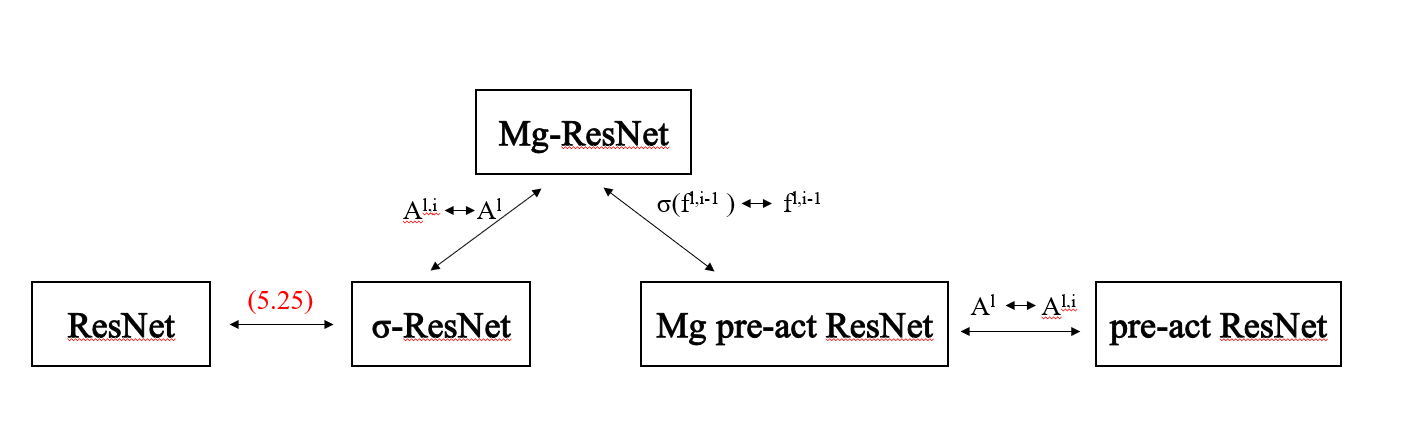
\includegraphics[width=1.0\textwidth]{Mgnetrelation} 
	\end{center}
	%\caption{Connections}
	\label{fig:mgnet}
\end{figure}
\vspace{-26pt}
%Because of the linearity of $\xi^{\ell,i}$, the above forms of iResNet and ResNet
%are equivalent to the previous as \eqref{dualmgnet} and \eqref{tilde-resnet}.
In this sense, these MgNet related models can be understood as
 models between pre-act ResNet and ResNet. And all these models can be
 understood as iteration in the data space as a dual relationship with
 feature space as MgNet.
 
 
The rationality of replacing  $A^{\ell,i}$ by layer independent $A^{\ell}$ may
be justified by the following theorem. 
\begin{theorem}\label{thm:CNN}
On each grid $\mathcal T_\ell$, 
\begin{enumerate}
	\item Any CNN model with
%	CNN and Mg-ResNet] 
	\begin{equation}
	\label{CNN1}
	f^{\ell,i} =   \chi^{\ell,i} \circ \sigma (f^{\ell,i-1}),
	\end{equation} 
	can be written as
	\begin{equation}\label{Res-CNN1}
	f^{\ell,i} = \sigma(f^{\ell,i-1}) - \xi^{\ell} \circ \sigma \circ \eta^{\ell,i} \circ\sigma ( f^{\ell,i-1}).
	\end{equation}
	\item Any CNN model with 
%	[CNN and ResNet] 
	\begin{equation}
	\label{CNN2}
	f^{\ell,i} =   \sigma\circ\chi^{\ell,i} (f^{\ell,i-1}).
	\end{equation}
	can be written as 
	\begin{equation}\label{Res-CNN2}
	f^{\ell,i} = \sigma\left(f^{\ell,i-1} - \xi^{\ell} \circ \sigma \circ \eta^{\ell,i}  ( f^{\ell,i-1})\right).
	\end{equation}
\end{enumerate}

%\begin{equation}
% \chi^{\ell,i}: \mathbb{R}^{n_\ell \times n_\ell \times c_\ell} 
% \mapsto \mathbb{R}^{n_\ell \times n_\ell \times c_\ell},
%\end{equation}
\end{theorem}
\begin{proof}
%	Without loss of generality, consider the classical CNN with 
%	\begin{equation}
%	f^{\ell,i} =   ({\rm id}  + \tilde \eta^{\ell,i} )\circ \sigma (f^{\ell,i-1}).
%	\end{equation}
Let use prove the first case as an example, 
the second case can be proven with the same process.

With similar structure in MgNet, we can take
\begin{equation}
\label{xi-cnn1}
\xi^{\ell}= \hat \delta^\ell :=  [\hat \delta_1, \cdots, \hat \delta_{{c_\ell}}],
\end{equation}
and 
\begin{equation}
\label{eta-ell}
\eta^{\ell,i} = [{\rm id}_{c_\ell}, -{\rm id}_{c_\ell}] \circ (\chi^{\ell,i} - {\rm id}_{c_\ell}).
\end{equation}
Here 
\begin{equation}
{\rm id}_{c_\ell}: \mathbb{R}^{n_\ell \times n_\ell \times c_\ell} 
\mapsto \mathbb{R}^{n_\ell \times n_\ell \times c_\ell},
\end{equation}
is the identity map and 
\begin{equation}
\hat \delta_k :  \mathbb{R}^{n_\ell \times n_\ell \times 2c_\ell} 
\mapsto \mathbb{R}^{n_\ell \times n_\ell},
\end{equation}
with 
\begin{equation}\label{eq:hatdelta}
\hat \delta_k([X ,Y]) = -([X]_k + [Y]_k),
\end{equation}
for any $X, Y \in \mathbb{R}^{n_\ell \times n_\ell \times c_\ell}$ 
and $[X,Y] \in \mathbb{R}^{n_\ell \times n_\ell \times 2c_\ell} $.


	First, we see that $\eta^{\ell,i}$ with the above 
	form is a convolution from $\mathbb{R}^{n_\ell \times n_\ell \times c_\ell}$
	to  $\mathbb{R}^{n_\ell \times n_\ell \times 2c_\ell}$.
	Following the identity
	\begin{equation}
	ReLU(x) + ReLU(-x) = x,
	\end{equation}
	and the definition of $\xi^{\ell}$ i.e. 
	\begin{equation}
	\xi^{\ell} = \hat \delta^\ell,
	\end{equation}
	as a special case in MgNet. 
	For more details, we can give a exact form of 
	$\hat \delta_k$ as in \eqref{eq:hatdelta} with
	\begin{equation}
	\hat \delta_k = [0, \cdots,0, -\delta, \cdots 0;  0, \cdots,0, -\delta, \cdots 0],  \quad k = 1:{c_\ell},
	\end{equation}
	where $\delta$ is the identity kernel during one channel.
	
	At last, we have
	\begin{align}
	\left[\xi^{\ell} \circ \sigma \circ [{\rm id}_{c_\ell}, -{\rm id}_{c_\ell}] (x) \right]_k &=  \left[\xi^{\ell} \circ \sigma \circ [x, -x]  \right]_k, \\
	&= \hat \delta_k ( [\sigma(x), \sigma(-x)]),  \\
	&= -\delta([\sigma(x)]_k) - \delta([\sigma(-x)]_k),\\
	&=-( \sigma([x]_k)+ \sigma(-[x]_k)) , \\
	&=  -[x]_k
	\end{align}
	Thus to say,
	\begin{equation}
	\xi^{\ell} \circ \sigma \circ [{\rm id}_{c_\ell}, -{\rm id}_{c_\ell}]  = -{\rm id}_{c_\ell}.
	\end{equation}
	Then the modified dual form of MgNet in \eqref{tilde-resnet} becomes
	\begin{align}
	f^{\ell,i} &= \sigma(f^{\ell,i-1}) - \xi^{\ell,i} \circ \sigma \circ \eta^{\ell,i} \circ\sigma ( f^{\ell,i-1}) , \\
	&=  \sigma(f^{\ell,i-1}) - \left( \xi^{\ell} \circ \sigma \circ [{\rm id}_{c_\ell}, -{\rm id}_{c_\ell}] \right) 
	\circ (\chi^{\ell,i} - {\rm id}_{c_\ell})\circ \sigma(f^{\ell,i-1})\\
	&=\sigma(f^{\ell,i-1}) + (\chi^{\ell,i} -{\rm id}_{c_\ell})\circ \sigma(f^{\ell,i-1}),  \\
	&=\chi^{\ell,i} \circ  \sigma (f^{\ell,i-1}).
	\end{align}
	This covers \eqref{Res-CNN1}.
\end{proof}


\begin{remark}
Theorems~\ref{thm:CNN} shows that general CNN in
the forms of either \eqref{CNN1} or \eqref{CNN2} can be written recast
as \eqref{Res-CNN1} or \eqref{Res-CNN2} with the data-feature mapping 
$A^\ell=\xi^\ell$ that is not only independent of the layers, but is
actually given a priori as in \eqref{xi-cnn1}.  In
view of Theorems~\ref{thm:mgnet1} and \ref{thm:mgnet2}, the classic
CNN models can be essentially recovered from MgNet by choosing
$\xi^\ell$ a priori as in  \eqref{xi-cnn1}.  Since
the classic CNN models have been extensively tested to be successful,
the more general MgNet with more general $\xi^\ell$ (to be trained)
are expected to be more efficient than the classic CNN models. 
\end{remark}

%At last we have the next relation:
%\input{MgNet-relation.tex}